\documentclass[a4paper,12pt,twoside,openany]{report}
%
% Wzorzec pracy dyplomowej
% J. Starzynski (jstar@iem.pw.edu.pl) na podstawie pracy dyplomowej
% mgr. inż. Błażeja Wincenciaka
% Wersja 0.1 - 8 października 2016
%
\usepackage{polski}
\usepackage{helvet}
\usepackage[T1]{fontenc}
\usepackage{anyfontsize}
\usepackage[utf8]{inputenc}
\usepackage[pdftex]{graphicx}
\usepackage{tabularx}
\usepackage{array}
\usepackage[polish]{babel}
\usepackage{subfigure}
\usepackage{amsfonts}
\usepackage{verbatim}
\usepackage{indentfirst}
\usepackage[pdftex]{hyperref}


% rozmaite polecenia pomocnicze
% gdzie rysunki?
\graphicspath{ {rys/} }
% oznaczenie rzeczy do zrobienia/poprawienia
\newcommand{\TODO}{\textbf{TODO}}


% wyroznienie slow kluczowych
\newcommand{\tech}{\texttt}

% na oprawe (1.0cm - 0.7cm)*2 = 0.6cm
% na oprawe (1.1cm - 0.7cm)*2 = 0.8cm
%  oddsidemargin lewy margines na nieparzystych stronach
% evensidemargin lewy margines na parzystych stronach
\def\oprawa{1.05cm}
\addtolength{\oddsidemargin}{\oprawa}
\addtolength{\evensidemargin}{-\oprawa}

% table span multirows
\usepackage{multirow}
\usepackage{enumitem}    % enumitem.pdf
\setlist{listparindent=\parindent, parsep=\parskip} % potrzebuje enumitem

%%%%%%%%%%%%%%% Dodatkowe Pakiety %%%%%%%%%%%%%%%%%
\usepackage{prmag2017}   % definiuje komendy opieku,nrindeksu, rodzaj pracy, ...
\usepackage{xspace}

%%%%%%%%%%%%%%% Strona Tytułowa %%%%%%%%%%%%%%%%%
% To trzeba wypelnic swoimi danymi
\title{Aplikacja do rozpoznawania emocji w sygnale mowy}

% autor
\author{Wojciech Decker}
\nrindeksu{252545}


\opiekun{dr inż. Andrzej Majkowski}
\konsultant{prof. Dzielny Konsultant}  % opcjonalnie
\terminwykonania{1 września 2017} % data na oświadczeniu o samodzielności
\rok{2017}


% Podziekowanie - opcjonalne
\podziekowania{\noindent
{\Large Podziękowania}
\bigskip

Dziękujemy bardzo serdecznie wszystkim, a w szczególności Rodzinom i~Unii Europejskiej...

\bigskip

{\raggedleft
Zdolny Student i Pracowity Kolega

}

}

% To sa domyslne wartosci
% - mozna je zmienic, jesli praca jest pisana gdzie indziej niz w ZETiIS
% - mozna je wyrzucic jesli praca jest pisana w ZETiIS
%\miasto{Warszawa}
%\uczelnia{POLITECHNIKA WARSZAWSKA}
%\wydzial{WYDZIAŁ ELEKTRYCZNY}
%\instytut{INSTYTUT ELEKTROTECHNIKI TEORETYCZNEJ\linebreak[1] I~SYSTEMÓW INFORMACYJNO-POMIAROWYCH}
\zaklad{ZAKŁAD SYSTEMÓW INFORMACYJNO POMIAROWYCH}
%\kierunekstudiow{INFORMATYKA}

% domyslnie praca jest inzynierska, ale po odkomentowaniu ponizszej linii zrobi sie magisterska
\pracamagisterska
%%% koniec od P.W

\opinie{%
\newpage
\begin{center}
 {\large\bf  Opinia} \\
o pracy dyplomowej magisterskiej wykonanej przez dyplomanta\\
{\bf Zdolnego Studenta i Pracowitego Kolegę} \\
 Wydział Elektryczny, kierunek Informatyka,  Politechnika Warszawska\\
Temat pracy\\
\textit{\bf
TYTUŁ PRACY DYPLOMOWEJ
}\\
\end{center}
\medskip
\noindent
Promotor: {\bf dr inż. Miły Opiekun}\\
Ocena pracy dyplomowej: {\bf bardzo dobry}

\medskip

\centerline{\bf Treść opinii}
   Celem pracy dyplomowej panów dolnego Studenta i Pracowitego Kolegi  było
opracowanie systemu pozwalającego symulować  i opartego o oprogramowanie o
otwartych źródłach (ang. Open Source). Jak piszą Dyplomanci, starali się opracować
system, który łatwo będzie dostosować do zmieniających się dynamicznie wymagań,
będzie miał niewielkie wymagania sprzętowe i umożliwiał dalszą łatwą rozbudowę oraz
dostosowanie go do potrzeb.
Przedstawiona do recenzji praca składa się z krótkiego wstępu jasno i
wyczerpująco opisującego oraz uzasadniającego cel pracy, trzech rozdziałów (2-4)
zawierających opis istniejących podobnych
rozwiązań, komponentów rozpatrywanychjako kandydaci do
tworzonego systemu i wreszcie zagadnień wydajności wirtualnych
rozwiązań. Piąty rozdział to opis przygotowanego przez
Dyplomantów środowiska obejmujący opis konfiguracji
środowiska oraz przykładowe ćwiczenia laboratoryjne. Ostatni
rozdział pracy to opis możliwości dalszego
rozwoju projektu. W ramach przygotowania pracy Dyplomanci zebrali i przedstawili w
bardzo przejrzysty sposób duży zasób informacji, co świadczy o dobrej orientacji
w nowoczesnej i ciągle intensywnie rozwijanej tematyce stanowiącej
zakres pracy i o umiejętności przejrzystego przedstawienia tych
wyników. Praca zawiera dwa dodatki, z których pierwszy obejmuje wyniki
eksperymentów i badań nad wydajnością, a drugi to źródła
skryptów budujących środowisko.

 Dyplomanci dość
dobrze zrealizowali postawione przed nimi zadanie,
wykazali się więc umiejętnością zastosowania w praktyce wiedzy
przedstawionej w rozdziałach 2-4.  Uważam, że cele postawione w założeniach pracy zostały pomyślnie
zrealizowane. Proponuję ocenę bardzo dobrą (5).

\vskip 1cm
{
\raggedleft
(data, podpis)\kern1cm

}
\newpage
\newpage
\begin{center}
 {\large\bf  Recenzja } \\
pracy dyplomowej magisterskiej wykonanej przez dyplomanta\\
{\bf Zdolnego Studenta i Pracowitego Kolegę} \\
 Wydział Elektryczny, kierunek Informatyka,  Politechnika Warszawska\\
Temat pracy\\
\textit{\bf
TYTUŁ PRACY DYPLOMOWEJ
}\\
\end{center}
\medskip
\noindent
Recenzent: {\bf prof. nzw. dr hab. inż. Jan Surowy}\\
Ocena pracy dyplomowej: {\bf bardzo dobry}
\medskip


\centerline{\bf Treść recenzji}
   Celem pracy dyplomowej panów dolnego Studenta i Pracowitego Kolegi  było
opracowanie systemu pozwalającego symulować  i opartego o oprogramowanie o
otwartych źródłach (ang. Open Source). Jak piszą Dyplomanci, starali się opracować
system, który łatwo będzie dostosować do zmieniających się dynamicznie wymagań,
będzie miał niewielkie wymagania sprzętowe i umożliwiał dalszą łatwą rozbudowę oraz
dostosowanie go do potrzeb.
Przedstawiona do recenzji praca składa się z krótkiego wstępu jasno i
wyczerpująco opisującego oraz uzasadniającego cel pracy, trzech rozdziałów (2-4)
zawierających bardzo solidny i przejrzysty opis: istniejących podobnych
rozwiązań (rozdz. 2), komponentów rozpatrywanychjako kandydaci do
tworzonego systemu (rozdz. 3) i wreszcie zagadnień wydajności wirtualnych
rozwiązań, zwłaszcza w kontekście współpracy  kilku elementów
 sieci (rozdział 4). Piąty rozdział to opis przygotowanego przez
Dyplomantów środowiska obejmujący opis konfiguracji
środowiska oraz przykładowe ćwiczenia laboratoryjne (5 ćwiczeń). Ostatni, szósty
rozdział pracy to krótkie zakończenie, które wylicza także możliwości dalszego
rozwoju projektu. W ramach przygotowania pracy Dyplomanci zebrali i przedstawili w
bardzo przejrzysty sposób duży zasób informacji o narzędziach, Rozdziały 2, 3 i 4 świadczą o dobrej orientacji
w nowoczesnej i ciągle intensywnie rozwijanej tematyce stanowiącej
zakres pracy i o umiejętności syntetycznego, przejrzystego przedstawienia tych
wyników. Drobne  mankamenty tej części pracy to zbyt skrótowe omawianie
niektórych zagadnień technicznych, zakładające dużą początkową wiedzę czytelnika
i dość niestaranne podejście do powołań na źródła.
Utrudnia to w pewnym stopniu czytanie pracy i zmniejsza jej wartość dydaktyczną
(a ta zdaje się być jednym z celów Autorów), ale jest zrekompensowane zawartością
merytoryczną. Praca zawiera dwa dodatki, z których pierwszy obejmuje wyniki
eksperymentów i badań nad wydajnością, a drugi to źródła
skryptów budujących środowisko. Praca
zawiera niestety dość dużą liczbę drobnych błędów redakcyjnych, ale nie wpływają
one w sposób istotny na na jej czytelność i wartość. W całej pracy przewijają
się samodzielne, zdecydowane wnioski Autorów, które są wynikiem własnych i
oryginalnych badań.  Rozdział 5 i dodatki pracy przekonują mnie, że Dyplomanci dość
dobrze zrealizowali postawione przed nimi zadanie. Pozwala to stwierdzić, że
wykazali się więc także umiejętnością zastosowania w praktyce wiedzy
przedstawionej w rozdziałach 2-4. Kończący pracę rozdział szósty świadczy o
dużym (ale moim zdaniem uzasadnionym) poczuciu własnej wartości i jest
świadectwem własnego, oryginalnego spojrzenia na tematykę przedstawioną w pracy
dyplomowej. Uważam, że cele postawione w założeniach pracy zostały pomyślnie
zrealizowane. Proponuję ocenę bardzo dobrą (5).

\vskip 1cm
{
\raggedleft
(data, podpis)\kern1cm

}
}

\streszczenia{
\newpage
\begin{center}
\large \bf
TYTUŁ PRACY DYPLOMOWEJ
\end{center}

\section*{Streszczenie}
Praca składa się z krótkiego wstępu jasno i
wyczerpująco opisującego oraz uzasadniającego cel pracy, trzech rozdziałów (2-4)
zawierających opis istniejących podobnych
rozwiązań, komponentów rozpatrywanychjako kandydaci do
tworzonego systemu i wreszcie zagadnień wydajności wirtualnych
rozwiązań. Piąty rozdział to opis  środowiska obejmujący opis konfiguracji
środowiska oraz przykładowe ćwiczenia laboratoryjne. Ostatni
rozdział pracy to opis możliwości dalszego
rozwoju projektu. 

\bigskip
{\noindent\bf Słowa kluczowe:} praca dyplomowa, LaTeX, jakość

\vskip 2cm


\begin{center}
\large \bf
THESIS TITLE
\end{center}

\section*{Abstract}
This thesis presents a novel way of using a novel algorithm to solve complex
problems of filter design. In the first chapter the fundamentals of filter design
are presented. The second chapter describes an original algorithm invented by the
authors. Is is based on evolution strategy, but uses an original method of filter
description similar to artificial neural network. In the third chapter the implementation
of the algorithm in C programming language is presented. The fifth chapter contains results
of tests which prove high efficiency and enormous accuracy of the program. Finally some
posibilities of further development of the invented algoriths are proposed.

\bigskip
{\noindent\bf Keywords:} thesis, LaTeX, quality

\vfill
}
\newcommand{\ang}[1]{\textit{(ang. #1)}}
\newcommand{\MATLAB}{\textsc{Matlab}\xspace}

\begin{document}
    \maketitle
    %-----------------
    % Wstęp
    %-----------------
    \chapter{Wstęp}
    \label{ch:wstep}
    % krótka definicja emocji
    Emojce to stany ludzkiego umysłu.
    Powstają w odpowiedzi na zdarzenie, są ukierunkowane i krótrkotrwałe.
    Różnią się intensywnością i zabarwieniem.
    Wpływają na interpretację bodżców z otoczenia,
    myśli a w konsekwencji mają istotny wpływ na zachowanie i reakcje.

    % informacje zakodowane w mowie
    Mowa jest nośnikiem informacji wykorzystywanym w komunikacji międzyludzkiej,
    oraz pomiędzy człowiekiem i komputerem \ang{Human-Computer Interaction}.
    Komunikat głosowy składa się z treści językowej,
    którą można zapisać w formie tekstu,
    oraz akustycznej, która również opisuje wypowiedź takie jak:
    drżący ze strachu głos, czy ciężki oddech świadczący o gniewie.

    % Zastosowanie maszynowego rozpoznawania emocji
    Rozpoznawanie emocji mówcy jest istotne w aplikacjach wykorzystujących mowę w komunikacji człowiek-maszyna.
    Zwłaszcza, jeśli odpowiedź systemu jest uzależniona od nastroju człowieka.
    Klasyfikacja emocji wypowiedzi jest wykożystywana w terapiach,
    gdzie terapełta wspiera się maszyną w odczytywaniu emocji pacjęta.
    Systemy tłumaczenia mszynowego mowy mogą wykożystać informacje mówiące o kontekście wypowiedzi i stanie mówcy.
    Telefoniczne centra obsługi klienta \ang{call center} rozpoznają stan klienta,
    oraz jego reakcję na ofertę prezentowaną przez konsultanta.

    % Jaki jest cel?
    Celem pracy jest przybliżenie tematyki komputerowego rozpoznawania mowy,
    przegląd wykorzystywanych narzędzi, oraz ocena znanych rozwiązań.
    Produktem końcowym będzie aplikacja komputerowa rozpoznająca emocje w sygnale mowy.
    W trakcje tworzenia pracy zostanie dokonana analiza znanych rozwiązań tego zagadnienia.
    Następnie zostanie opracowany schemat aplikacji, bzujący na poprzednich badaniach,
    pozwalający stworzyć aplikację w warunkach powstawania pracy magisterskiej.
    Kolejnym etapem będzie implementacja aplikacji w srodowisku MATLAB.
    Na zakończenie zostaną przeprowadzone testy aplikacji,
    analiza wyników i prezentacja wniosków.

    \chapter{Omówienie problemu rozpoznawania emocj}
    \label{ch:omowienie_problemu}

    \section{Ogólny algorytm rozpoznawania emocji}
    \label{sec:ogol}
    \begin{figure}[h]
        \centering
        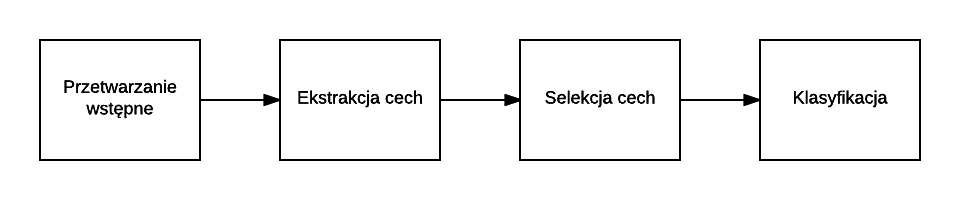
\includegraphics[width=0.5\textwidth]{generic_schema}
        \caption{Schemat systemu rozpoznawania emocji}
    \end{figure}

    \section{Przetwarzanie wstępne}
    Wejściem jest plik audio z zapisem sygnału mowy.
    Przed rozpoczęciem przetwarzania musi zostać podzielone na ramki,
    na którch będą wykonywane operacje w późniejszych etapach.

    Sygał odczytany z pliku przefiltrowano wybierną funkcją operatorową(ang.  rational transfer function).
    Przyjmując współczynniki numeratora (b) i denominatora(a)
    $b = 0.03$ $a = 1$  % funkcja filter z matlaba

    Sygnał jest podzielony na ramki o stałej długości.
    Każda ramka zawierała 200 próbek.
    Ramki nie nachodziły na siebie.
    Każda ramka została przetworzona przez okno Hamminga \ref{eq:hamming}.

    \begin{figure}
        \label{eq:hamming}
        \[w(n) = \alpha - \beta \cos(\frac{2 \pi n}{N -1})\]
        \caption{Okno Hamminga}
    \end{figure}

    Przyjęto wartości parametrów $\alpha = 0.54$ $\beta = 0.46$


    \section{Ekstrakcja cech}
    Przyjmując za dane wejściowe sygnał podzielony na ramki przeprowadzono ekstrakcję cech z sygnału.
    Każdą ramkę przetworzono obliczając cechy:
    \begin{enumerate}
        \item MFCC (7 pierwszych współczynników)
        \item energia ramki
        \item częstotliwość podstawowa (dla całego sygnału)
        \item formanty(pierwsze 4)
    \end{enumerate}
    \subsection{Opis współczyników}
    \subsubsection{MFCC}
    \subsubsection{Energia}
    \subsubsection{Częstotliwość podstawowa}
    \subsubsection{Formanta}
    \section{Selekcja cech}
    Współczynniki z ramek poddano analizie statystycznej.
    Dla każdej ramki obliczono:
    \begin{enumerate}
        \item średnią
        \item wariancję
        \item zakres
        \item wartość minimalną
        \item skośność
        \item kurtozę
    \end{enumerate}

    \section{Klasyfikacja}
    Wybrano siedem wartości opisujących każdą wypowiedź:
    \begin{enumerate}
        \item zakres pierwszego współczynnika MFCC
        \item średnia drugiej formanty
        \item minimalna szóstego współczynnika MFCC
        \item zakres tonu podstawowego
        \item minimalna siódmego współczynnika MFCC
        \item kurioza szóśtego współczynnika MFCC
        \item zakres drugiej formanty
    \end{enumerate}
    Klasyfikacji dokonano z wykorzystanie klasyfikatora najbliższych sąsiadów.
    Z wszystkich wypowiedzi 10\% zostało wykoryzstane jako dane testowe.

    \chapter{Analiza wybranych przypadków}

    \section{Badanie 1}

    \section{Badanie 2}
    \section{Badanie 3}

    \chapter{Opracowanie i implementacja algorytmu rozpoznawania emocji}
    \chapter{Testowanie poprawności działania aplikacji}
    \begin{thebibliography}{99}
        \addcontentsline{toc}{chapter}{Bibliografia}
        \bibitem{Stevens}{W. R. Stevens, G. R. Wright, ,,Biblia TCP/IP tom 1'', RM,
        1998.}
        Emotion recognition and affective computing on vocal social media
        \bibitem{Stevens}{W. R. Stevens, G. R. Wright, ,,Biblia TCP/IP tom 1'', RM,
        1998.}
        \bibitem{USDoD}{U. S. Department Of Defense, ,,Trusted Computer System
        Evaluation Criteria'', 1985.}
        \bibitem{FirstCC}{B. W. Lampson, ,,A note on the confinment problem'', w ,,Proc.
        of the Communications of the ACM'', październik 1973, numer 16:10,\newline
        strony 613-615.}
        \bibitem{PrisonersProblem}{G. J. Simmons, ,,The prisoners' problem and the
        subliminal channel'', w ,,Advances in Cryptology: Proceedings of Crypto 83 (D.
        Chaum, ed.)'', strony 51-67, Plenum Press, 1984.}
        \bibitem{Kerckhoff}{ A. Kerckhoffs, ,,La Cryptographie Militaire (Military
        Cryptography)'', J. Sciences Militaires, luty 1883.}
        \bibitem{Hanssen}{A. Havill, ,,The Spy Who Stayed Out In The Cold: The Secret
        Life of Double Agent Robert Hanssen'', St. Martin's Press, 2001.}
        \bibitem{schematKomunikacjiPrzypis}{C.Cachin, ,,An Information-Theoretic Model
        for Steganography'', w ,,Information and Computation'', 4 marzec 2004.}
        \bibitem{SweetyPresentation}{S.Chauhan, ,,Embedding Covert Channels into
        TCP/IP'', 7th Information Hiding Workshop, czerwiec 2005.}
        \bibitem{RFC793}{Information Sciences Institute, University of Southern
        California, ,,Transmission Control Protocol'', RFC793, wrzesień 1981.}
        \bibitem{RFC1323}{V. Jacobson, R. Braden, D. Borman, ,,TCP extensions for high
        performance'', RFC1323, maj 1992.}
        \bibitem{RFC1948}{S. Bellovin, ,,Defending against sequence number attacks.'',
        RFC1948, IETF, 1996.}
        \bibitem{RFC2960}{R. Stewart, Q. Xie, K. Morneault, C. Sharp, H. Schwarzbauer,
        T. Taylor, I. Rytina, M. Kalla, L. Zhang, V. Paxson, „Stream Control
        Transmission Protocol”, RFC2960, Network Working Group, październik 2000.}
        \bibitem{Rowland}{C. H. Rowland, ,,Covert Channels in the TCP/IP Protocol
        Suite'', First Monday, 1997. \newline
        \url{http://www.firstmonday.dk/issues/issue2\_5/rowland/}}
        \bibitem{LOKI}{Alhambra, daemon9, ,,Project Loki: ICMP Tunneling'', Phrack
        Magazine, Issue 49. \url{http://phrack.org}}
        \bibitem{LOKI2}{daemon9, ,,LOKI2'', Phrack Magazine, Issue 51.
        \url{http://phrack.org}}
        \bibitem{RWWWS}{van Hauser, Reverse WWW Shell, THC, The Hacker's
        Choice.\newline \url{www.thc.org}}
        \bibitem{CCdetectionSVM}{T. Sohn, J. Seo, J. Moon, ,,A Study on the Covert
        Channel Detection of TCP/IP Header Using Support Vector Machine'', Volume 2836
        of Lecture Notes in Computer Science., Springer-Verlag (2003) 313-324.}
        \bibitem{LOKIdetectionSVM}{T. Sohn, T. Noh, J. Moon, ,,Support Vector Machine
        Based ICMP Covert Channel Attack Detection'', Volume 2836 of Lecture Notes in
        Computer Science., Springer-Verlag, 2003, strony 461-464.}
        \bibitem{devcc}{J. Giffin, R. Greenstadt, P. Litwack, R. Tibbetts, ,,Covert
        messaging in TCP'', w Dingledine, Privacy Enhancing Technologies. Volume 2482 of
        Lecture Notes in Computer Science., Springer-Verlag (2002) 194-208.
        \url{http://www.mit.edu/\textasciitilde gif/covert-channel/}}
        \bibitem{ActiveWardens}{G. Fisk, M. Fisk, Ch. Papadopoulos, J. Neil,
        ,,Eliminating Steganography in Internet Traffic with Active Wardens'', 5th
        International Workshop on Information Hiding, październik 2002.}
        \bibitem{JR}{J. Rutkowska, ,,The Implementation of Passive Covert Channels in
        Linux Kernel'', Chaos Communication Congress, grudzień 2004.}
        \bibitem{LinuxNetwork}{Ch. Benvenuti, ,,Understanding Linux Network Internals'',
        O'Reilly,\newline grudzień 2005.}
        \bibitem{p55}{kossak, ,,Building Into The Linux Network Layer'', Phrack
        Magazine, Issue 55. \url{http://phrack.org}}
        \bibitem{ML}{Steven J.Murdoch and Stephen Lewis, ,,Embedding Covert Channels
        into TCP/IP'', University of Cambridge, Computer Laboratory,\newline 29 lipec
        2005.}
        \bibitem{NvsNN}{Eugene Tumoian, Maxim Anikeev, ,,Detecting NUSHU Covert Channels
        Using Neural Networks'', Taganrog State University of Radio Engineering,
        Department of Information Security.}
        \bibitem{p58}{mayhem, ,,IA32 Advanced Function Hooking'', Phrack
        Magazine,\newline Issue 58. \url{http://phrack.org}}
        \bibitem{p61}{bioforge, ,,Hacking the Linux Kernel Network Stack'', Phrack
        Magazine, Issue 61. \url{http://phrack.org}}
        \bibitem{kernelMEM}{Robert Love, ,,Kernel Korner - Allocating Memory in the
        Kernel'',\newline 1 grudzień 2003.}

    \end{thebibliography}

    \zakonczenie
    % wklejenie recenzji i opinii

\end{document}
%+++ END +++
%-----------------
% Historia
%-----------------
\section{Historia}
Pomimo, że pierwsze wzmianki o steganografii, a dokładnie o ukrytych kanałach w
odniesieniu do systemów informatycznych notuje się na lata siedemdziesiąte XX
wieku \cite{FirstCC}, to przykłady użycia steganografii sięgają starożytności. W
literaturze powtarzają się opisy przekazywania tajnej informacji poprzez
wytatuowanie jej na ogolonej głowie posłańca, który po odrośnięciu włosów był
wysyłany z mało znaczącą wiadomością do armii swojego dowódcy. Każdy kto natknął
się na posłańca miał wgląd do nieważnej wiadomości, niepodejrzewając nawet
istnienia sekretnej informacji w postaci tatuażu.

Przykłady z historii odnoszą się także do bardziej współczesnych czasów. Wiele z
metod steganografii było stosowanych podczas II Wojny Światowej (np.
mikro-kropki) a także w latach Zimnej Wojny. Wiadomo także, że wielu agentów
służb wywiadowczych, a szczególnie podwójnych agentów, przekazywało obcym
państwom informację wykorzystując steganografię. Przykładem może tu być sprawa
szpiega FBI Roberta Hanssena \cite{Hanssen}, który przy pomocy technik
steganograficzny przez około dekadę przekazywał tajne informacje służbom KGB.

Rozdziały \ref{sectionSteganografiaWObiektachMultimedialnych} oraz
\ref{chapterSteganografiaWRuchuTCPIP} opisują nowoczesne podejście do
steganografii wykorzystujące współczesne kanały informacyjne.
%-----------------
% Pojęcia
%-----------------
\section{Pojęcia}
W celu zdefiniowania kanału steganograficznego oraz opisania transmisji z
wykorzystaniem takiego kanału należy omówić jego części składowe:
\begin{itemize}
    \item dane do ukrycia, tajne dane - informacja jaką należy przesłać
    między uczestnikami komunikacji, tak aby strony trzecie nie miały do niej
    wglądu,
    \item dane nośne, wiadomość zakrywająca - wiadomość, w której ukryte
    zostaną tajne dane; przesyłanie wiadomości zakrywających musi być dozwolone w
    danym kanale informacyjnym i nie powinno wzbudzać podejrzeń,
    \item funkcja steganograficzna - funkcja przekształcająca dane do
    ukrycia oraz wiadomość zakrywającą w jedną połączoną wiadomość,
    \item dane z ukrytą wiadomością - dane zawierające ukrytą informację a
    jednocześnie wykazujące cechy danych nośnych,
    \item nadzorca komunikacji, wartownik - mechanizm mający pełen wgląd do
    wiadomości przekazywanej między stronami komunikacji, świadomy struktury
    komunikatów i potrafiący wykrywać występujące w nich anomalie,
    \item kanał komunikacyjny - kanał zestawiony pomiędzy nadawcą a
    odbiorcą, zapewniający przepływ informacji, do którego wgląd ma nadzorca
    komunikacji,
    \item odwrotna funkcja steganograficzna - funkcja przekształcająca dane
    z ukrytą wiadomością na tajne dane,
    \item klucz kryptograficzny - klucz znany tylko obu stronom komunikacji,
    służący do zabezpieczenia tajnej informacji metodami kryptografii symetrycznej
    przed ewentualnością złamania funkcji steganograficznej.
\end{itemize}
%-----------------
% Schemat komunikacji steganograficznej
%-----------------
\section{Schemat komunikacji steganograficznej}
\label{sectionSchematKomunikacjiSteganograficznej}
Podstawowy scenariusz, powszechny w literaturze na temat steganografii, odnosi
się do sytuacji opisanej w \cite{PrisonersProblem}. Dwóch więźniów (w naszym
przypadku Alicja(\tech{A}) i Bob(\tech{B})) zamknięci są w dwóch odrębnych
celach. Mogą się ze sobą kontaktować, jednak ich cała korespondencja przechodzi
przez ręce Wartownika (\tech{W}). Ma on pełen wgląd do przekazywanych
informacji, więc może przechwycić wszelkie przekazywane tajemnice, a dodatkowo w
razie podejrzeń może nie dopuścić do komunikacji\footnote{podejrzana informacja
jest tu analogią do stosowania kryptografii przez więźniów}. W takim przypadku w
celu przekazania ważnych informacji \tech{A} i \tech{B} muszą posłużyć się
pewnego rodzaju podstępem. Muszą tak sformułować treść przekazu, aby \tech{W}
nie rozróżnił ,,niegroźnej'' wiadomości od wiadomości z ukrytym przekazem.
Dlatego też przekazują wiadomość, w której prawdziwa treść możliwa jest do
odczytania po złożeniu kolejno każdej np. drugiej litery z każdego wyrazu.
\begin{figure}[!htbp]
    \begin{center}
        \centering
        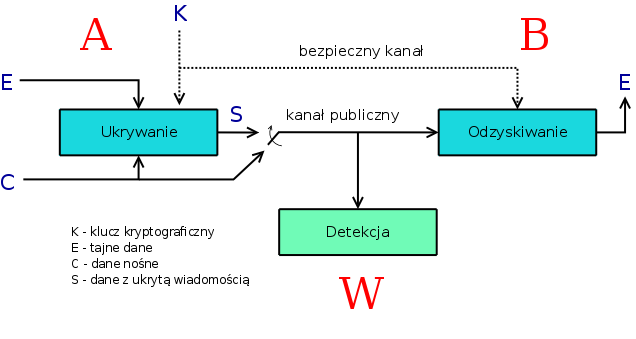
\includegraphics[scale=0.4]{\ImgPath/rys/schemat_komunikacji.png}
    \end{center}
    \caption{Schemat komunikacji steganograficznej}
    \label{schematKomunikacji}
\end{figure}

Przedstawioną tak sytuację pokazuje rysunek
\ref{schematKomunikacji}\footnote{sporządzony na podstawie
\cite{schematKomunikacjiPrzypis}, rysunek 1, strona 3}. \tech{A} próbuje
przesłać tajną informację \tech{E} do \tech{B}. Cała komunikacja odbywa się
przez kanał publiczny, kontrolowany przez \tech{W}. W celu ukrycia faktu
komunikacji \tech{A} stara się ukryć tajny przekaz w informacji \tech{C}. W celu
uzyskania skutecznej steganografii \tech{W} nie może rozróżnić informacji
poprawnej, nie zawierającej tajnych danych, od informacji \tech{S}, która
zawiera tajną informację. W celu dodatkowego zabezpieczenia przekazu, \tech{A} i
\tech{B} mogą korzystać z funkcji kryptograficznej zabezpieczającej przekazywane
informacje. Można tu wykorzystać metody kryptografii symetrycznej (ustalony
klucz kryptograficzny \tech{K}) lub niesymetrycznej (klucz publiczny
\tech{K}$_{pub}$ i klucz prywatny \tech{K}$_{pryw}$).

Stosowanie technik kryptograficznych wpływa na poprawę bezpieczeństwa
przesyłanej informacji, jednak należy pamiętać o nieporządnych cechach jakie
mogą one wywołać. W większości przypadków umieszczenie tajnej informacji
steganograficznej w przekazie wiąże się z zamianą istniejącej już nieważnej
części informacji. Jednak każda porcja usuniętej informacji może mieć pewną
charakterystyczną postać lub specyficzny histogram. Zastosowanie funkcji
kryptograficznej w stosunku do tajnej informacji zmienia ją, a wynikowy rozkład
bitów jest nieprzewidywalny i w większości przypadków różny od standardowych
histogramów określonych dla podmienianych części wiadomości.
%-----------------
% Stegoanaliza
%-----------------
\section{Stegoanaliza}
Stegoanaliza to nauka zajmująca się wykrywaniem istnienia ukrytych informacji w
kanałach komunikacyjnych. Nie zawsze prowadzi to do odkrycia dokładnej treści
ukrytego przekazu, a w większości przypadków polega jedynie na wskazaniu
istnienia ukrytego kanału steganograficznego.

Możliwość wykrycia kanału steganograficznego sprowadza się do analizy różnych
części wiadomości lub strumienia danych w celu wykrycia anomalii. Takie
podejście wynika z faktu, że tajna informacja ukryta jest w miejscach nie
przeznaczonych do przesyłania informacji lub na miejscu danych, które są w
pewien sposób nadmiarowe (np. dla zmysłów człowieka). Można wskazać dwa
podstawowe sposoby wykrywania anomalii:
\begin{itemize}
    \item pierwsze podejście opiera się na przebadaniu wszystkich części
    informacji (np. pól nagłówka TCP/IP), których struktura jest w pełni
    przewidywalna lub których wartości są zdefiniowane przez standardy lub
    powszechne praktyki; ważne jest także sprawdzenie czy występują wartości
    nadmiarowe oraz czy elementy sygnalizujące wystąpienie dodatkowych danych mają
    faktyczne pokrycie w danych,
    \item drugą metodą jest porównanie wartości części wiadomości (np. pól
    nagłówka TCP/IP) i zaklasyfikowanie ich jako prawdopodobnych lub nie dla danego
    systemu bądź protokołu; takie podejście może być stosowane do wartości ściśle
    określonych, takich jak wymienione w pierwszym punkcie, jednak można je także
    stosować do wartości które są pseudolosowe lub których histogram jest
    charakterystyczny; w celu realizacji tej metody warto posłużyć się sieciami
    neuronowymi takimi jak SVM i RSVM, zdolnymi rozpoznawać wzorce i separować dane.
\end{itemize}
%-----------------
% Metody tworzenia steganografii
%-----------------
\section{Metody tworzenia steganografii oraz rodzaje ukrytych kanałów}
Przesłanie danych za pomocą przekazu steganograficznego wiąże się w większości
przypadków z umieszczeniem dodatkowej informacji w wiadomości. Odbywa się to za
pomocą podmiany tej części wiadomości (nagłówka TCP/IP), która wykazuje cechy
nadmiarowości lub której (kontrolowana) zmiana nie prowadzi do przerwania
transmisji. Pewną podgrupą może być w tym przypadku wykorzystanie pól
oryginalnie pustych (zerowych) lub niewykorzystywanych w istniejących
implementacjach.

Kanały steganograficzne można podzielić na dwa zasadniczne
typy\cite{SweetyPresentation}:
\begin{itemize}
    \item kanał pojemnościowy (ang. storage channel) - informacja zawarta w
    częściach wiadomości, polach nagłówka,
    \item kanał czasowy (ang. timing channel) - informacja zawarta w czasach
    wystąpienia danych zdarzeń, np. przesłania pakietu TCP/IP.
\end{itemize}
W przypadku sieci pakietowych można także połączyć dwa typu kanałów
steganograficznych, tworząc kanał mieszany, w którym jeden z typów (np.
pojemnościowy) będzie wykorzystywany do przekazywania informacji, a drugi (np.
czasowy) do sygnalizacji tego zdarzenia.

Większość opracowanych programów służących do przesyłania danych z
wykorzystaniem steganografii opiera się na kanałach pojemnościowych. Wynika to z
faktu, że kanały czasowe narzucają pewne ograniczenia na generację pakietów
TCP/IP przez co ich wykrycie staje się prostsze.

Dodatkowo należy zauważyć, że w sieciach pakietowych można skonstruować
abstrakcyjny kanał steganograficzny, w którym do przesyłania tajnych danych
lub/i obsługi protokołu steganograficznego wykorzystywane są różne pola
nagłówka. Zmiana wykorzystania danego pola może być dynamiczna, zależna od
wymaganej przepustowości lub w celu zminimalizowania wykrycia kanału
steganograficznego.
%-----------------
% Cechy kanału steganograficznego
%-----------------
\section{Cechy kanału steganograficznego}
Każdy kanał steganograficzny posiada trzy cechy, które decydują o jego
przydatności w danej sytuacji:
\begin{enumerate}
    \item pojemność (przepustowość) - określa jaką porcję informacji możemy
    przesłać w danej wiadomości nośnej; w przypadku steganografii w TCP/IP, wyrażana
    jest w bitach na sekundę, bitach na pakiet lub bitach na sesję TCP;
    przepustowość odgrywa ważną rolę w przypadku konieczności przekazania dużej
    ilości informacji, jednak należy pamiętać, że to przeważnie prowadzi do
    ułatwionej detekcji steganografii,
    \item bezpieczeństwo - określa jak łatwo jest uzyskać dostęp do
    przekazywanej tajnej informacji w przypadku poznania mechanizmu tworzenia
    przekazu steganograficznego; dodatkowym mechanizmem zwiększającym bezpieczeństwo
    może być używanie znanych tylko sobie zmiennych pseudolosowych lub modyfikacji
    algorytmu\footnote{jest to znane jako ,,bezpieczeństwo przez zatajenie'' (ang.
    security through obscurity) i powinno być używane tylko jako dodatkowy element
    systemu zabezpieczeń},
    \item krzepkość (ang. robustness) - określa stopień w jakim możemy
    zmodyfikować przekaz nie uszkadzając zawartej w nim informacji
    steganograficznej; niestety w przypadku steganografii naruszenie kanału (pola)
    zawierającego przekaz steganograficzny przeważnie wiąże się z utratą tajnego
    przekazu.
\end{enumerate}

%-----------------
% Steganografia w obiektach multimedialnych
%-----------------
\section{Steganografia w obiektach multimedialnych}
\label{sectionSteganografiaWObiektachMultimedialnych}
Pomimo, że steganografia ma zastosowanie prawie w każdej formie komunikacji, w
latach 90-tych zyskała ona powodzenie jako technika ukrywania informacji w
obiektach multimedialnych. Wynika to przede wszystkim z powszechności tego
rodzaju przekazu, jego rozmiarów oraz prostoty obsługi programów do ukrywania
informacji w obiektach multimedialnych, takich jak obraz, dźwięk i wideo.
Dodatkowym atutem przy zastosowaniu tych metod jest stosunek ukrytej informacji
do oryginalnego przekazu, sięgający w ekstremalnych sytuacjach 50\%, bez
zauważalnego pogorszenia się jakości przekazywanych danych.

Użycie steganografii w treściach multimedialnych sprowadza się do takiego
manipulowania danymi, aby plik wynikowy zawierał dodatkowe informacje, a
jednocześnie nie był rozróżniany przez zmysły człowieka w porównaniu z
oryginałem.

Jedną z najszerzej omawianych form steganografii w obiektach multimedialnych
jest ukrywanie informacji w plikach graficznych. Istnieje wiele rozwiązań,
zarówno bezpłatnych, o otwartym kodzie jak i komercyjnych. Przykładami mogą tu
być takie programy jak Outguess, JPHide, StegHide. Istnieją różne techniki
ukrywania informacji w plikach graficznych. Najprostszym rozwiązaniem jest
podmiana najmniej znaczących bitów opisujących kolor danego piksela. Możliwe
jest też zastosowanie dyskretnej transformaty kosinusowej.

W przypadku wybrania jako wiadomości nośnej pliku audio, możemy także zastosować
metodę podmiany najmniej znaczących bitów. Dodatkowo stosowane są metody
ukrywania tajnych wiadomości poprzez rozszerzanie spektrum danego nagrania, czy
też dodawanie echa. Przykładem narzędzia do tworzenia wiadomości
steganograficznych może być UnderMP3Cover, MP3Stego czy
S-Tools\footnote{\url{http://www.stegoarchive.com}}.

Kolejnym przykładem wykorzystania jako pliku nośnego obiektu multimedialnego
jest plik wideo. Dodatkowa informacja może być przekazana przy użyciu dyskretnej
transformaty kosinusowej. Jako przykładowe implementacje można podać StegoVideo.

Istnieje kilka technik umożliwiających wykrycie lub usunięcie steganografii
zastosowanej w obiektach multimedialnych. Pierwszym podejściem, choć przeważnie
trudnym do zastosowania, jest użycie oryginalnego pliku jako wzorca do
porównania z przechwyconą wersją. W przypadku plików graficznych lub wideo
możliwe jest użycie analizatorów statystycznych, które mogą wykryć anomalie
występujące w histogramach tych wiadomości.

Zamiast wykrywać istnienie steganografii, częstym podejściem jest jej
ograniczanie lub ,,ślepe'' usuwanie z wiadomości tych danych, które mogą być
nośnikiem kanału steganograficznego. W przypadku plików multimedialnych
najlepszym sposobem uzyskania takiego efektu jest przekodowanie pliku na inny
standard i powrót do standardu wejściowego. Przeważnie zmiany w jakości plików
są niezauważalne, a użycie konwersji sprowadza się do takiej zmiany bitów, która
niszczy zawartą w nich steganografię.

W przypadku plików multimedialnych użycie steganografii jest pomocne w ochronie
praw autorskich, przez stosowanie jej jako cyfrowych znaków wodnych. Niestety,
tak jak zostało to wcześniej przedstawione w trakcie konwersji wiele z
zakodowanej informacji ginie bezpowrotnie. Skutkiem tego może być pogorszenie
jakości pliku multimedialnego, ale także usunięcie z niego cyfrowego znaku
wodnego.

Itd., itd., itd. ...

\chapter{Steganografia w ruchu TCPIP}
\label{chapterSteganografiaWRuchuTCPIP}

Itd., itd., itd ...

%-----------------
% Wnioski 
%-----------------
\chapter{Wnioski}

Protokół TCP/IP jest najbardziej rozpowszechnionym i używanym protokołem
komunikacji między systemami w sieci Internet oraz w sieciach intranet. Niestety
został on opracowany na początku lat siedemdziesiątych, gdy problemy
bezpieczeństwa informacji nie stały na pierwszym miejscu. Ciągły wzrost działań
przestępczych w sieci Internet, w tym wymiana nielegalnych treści, prowadzi do
stosowania coraz to nowszych technik zabezpieczających. Z tego względu obserwuje
się działania mające na celu wprowadzenie tajnej komunikacji między przejętymi
systemami, tak aby nie wzbudzić ostrzeżeń w analizatorach sieciowych. Taka
ukryta komunikacja odbywa się z wykorzystaniem steganografii.

Wprowadzenie steganografii do niskich warstwach stosu TCP/IP umożliwia obejście
wielu filtrów nałożonych na warstwy wyższe. Większość sieci oparta jest na
protokołach rodziny TCP/IP, przez co nie można zabronić ich używania. Możliwa
jest jedynie kontrola poprawności semantyki protokołów TCP/IP, a także
ewentualna ingerencja w przekazywane wartości, z uwzględnieniem stanowości
niektórych pól.

Opracowany schemat generacji początkowych numerów sekwencyjnych w jak najlepszy
sposób odzwierciedla oryginalny proces zachodzący w stosie sieciowym systemu
Linux. W większości przypadków występujących w rzeczywistych sieciach i
systemach, numery wygenerowane przy pomocy \tech{Shushi} nie byłyby rozróżnialne
od numerów wygenerowanych przez stos sieciowy systemu.

Jeżeli proces generacji wartości użytych do przekazania danych
steganograficznych zostanie oparty o oryginalne mechanizmy używane do ich
generacji, to pasywny analizator sieciowy nie będzie w stanie wykryć istnienia
anomalii. Różnice możliwe są do zaobserwowania w przypadku zaistnienia
specyficznych sytuacji występujących dla danej implementacji protokołu. W
przypadku zastosowania pasywnego analizatora wymaga to jednak oczekiwania na
taką sytuację. Z przeprowadzonych testów wynika, że lepszym podejściem jest
zastosowanie analizatorów aktywnych, które posiadają wiedzę na temat testowanych
systemów oraz ich chrakterystycznych cech implementacji. Skonstruowanie takiego
analizatora jest zadaniem stosunkowo prostym a daje bardzo wysoką skuteczność.

Z przeprowadzonych testów wynika, że celowe jest prowadzenie dalszych prac w
następujących obszarach:
\begin{itemize}
    \item dokładniejszy mechanizm generacji wartości mikrosekund
    \item wprowadzenie algorytmów zdolnych wykryć i uniemożliwić działanie
    analizatora aktywnego
\end {itemize}

Jeżeli powyższe punkty nie zostaną spełnione, analizatory aktywne będą w stanie
wykryć istnienie modułu steganograficznego opartego na początkowych numerach
sekwencyjnych.

\begin{tabular}{c|cc}
    pierwsza kolumna & druga & trzecia \\ \hline
    1 & 2 & 3 \\
    a & b & c \\
\end{tabular}

\begin{equation}
    E = m c^2 \label{einstein}
\end{equation}

Rozwój opracowanego rozwiązania steganograficznego jest możliwy poprzez
wprowadzenie elementów -- patrz wzór (\ref{einstein}) -- jak:
\begin{itemize}
    \item obsługa innych, przyszłościowych protokołów sieciowych, takich jak SCTP
    (ang. Stream Control Transmission Protocol)\cite{RFC2960}
    \item zapewnienie dwustronnej komunikacji z wykorzystaniem numerów
    potwierdzenia \tech{ACK}
    \item przeniesienie implementacji do innych systemów operacyjnych
\end{itemize}

Wraz ze wzrostem przepustowości urządzeń sieciowych (obecnie 10Gb/s i więcej)
wzrasta problem analizy przepływających danych w czasie rzeczywistym.
Analizatory sieciowe muszą w coraz krótszym czasie zbadać coraz większy strumień
danych (miliony pakietów na sekundę). Jednak problem wzrostu prędkości sieci
utrudnia zadanie także osobom implementującym kanały steganograficzne w
protokole TCP/IP. Coraz więcej operacji wyższych warstw stosu sieciowego
przenoszonych jest do układów scalonych interfejsów sieciowych. Taka technologia
znana jest pod skrótem TOE (ang. TCP Offload Engine) i odnosi się przede
wszystkim do sprzętowej generacji sum kontrolnych oraz mechanizmu TSO (ang. TCP
segmentation offload). W następnych latach spodziewane jest przenoszenie
kolejnych elementów stosu sieciowego TCP/IP do implementacji sprzętowych.

Ze względu na rozwój systemów zabezpieczających ruch sieciowy oraz wzrost
bezpieczeństwa systemów operacyjnych, w kolejnych latach wzrośnie także
wykorzystanie technik steganograficznych przez grupy przestępcze działające w
ramach Internetu. Z tego powodu poznanie technik steganograficznych oraz
wypracowanie metod obrony i wykrywania takiej komunikacji jest bardzo ważne.

%-----------------
% Dodatki 
%-----------------
\appendix
\chapter{Porównanie numerów ISN jądra Linux i modułu Shushi}
\begin{figure}[!htbp]
    \begin{center}
        \centering
        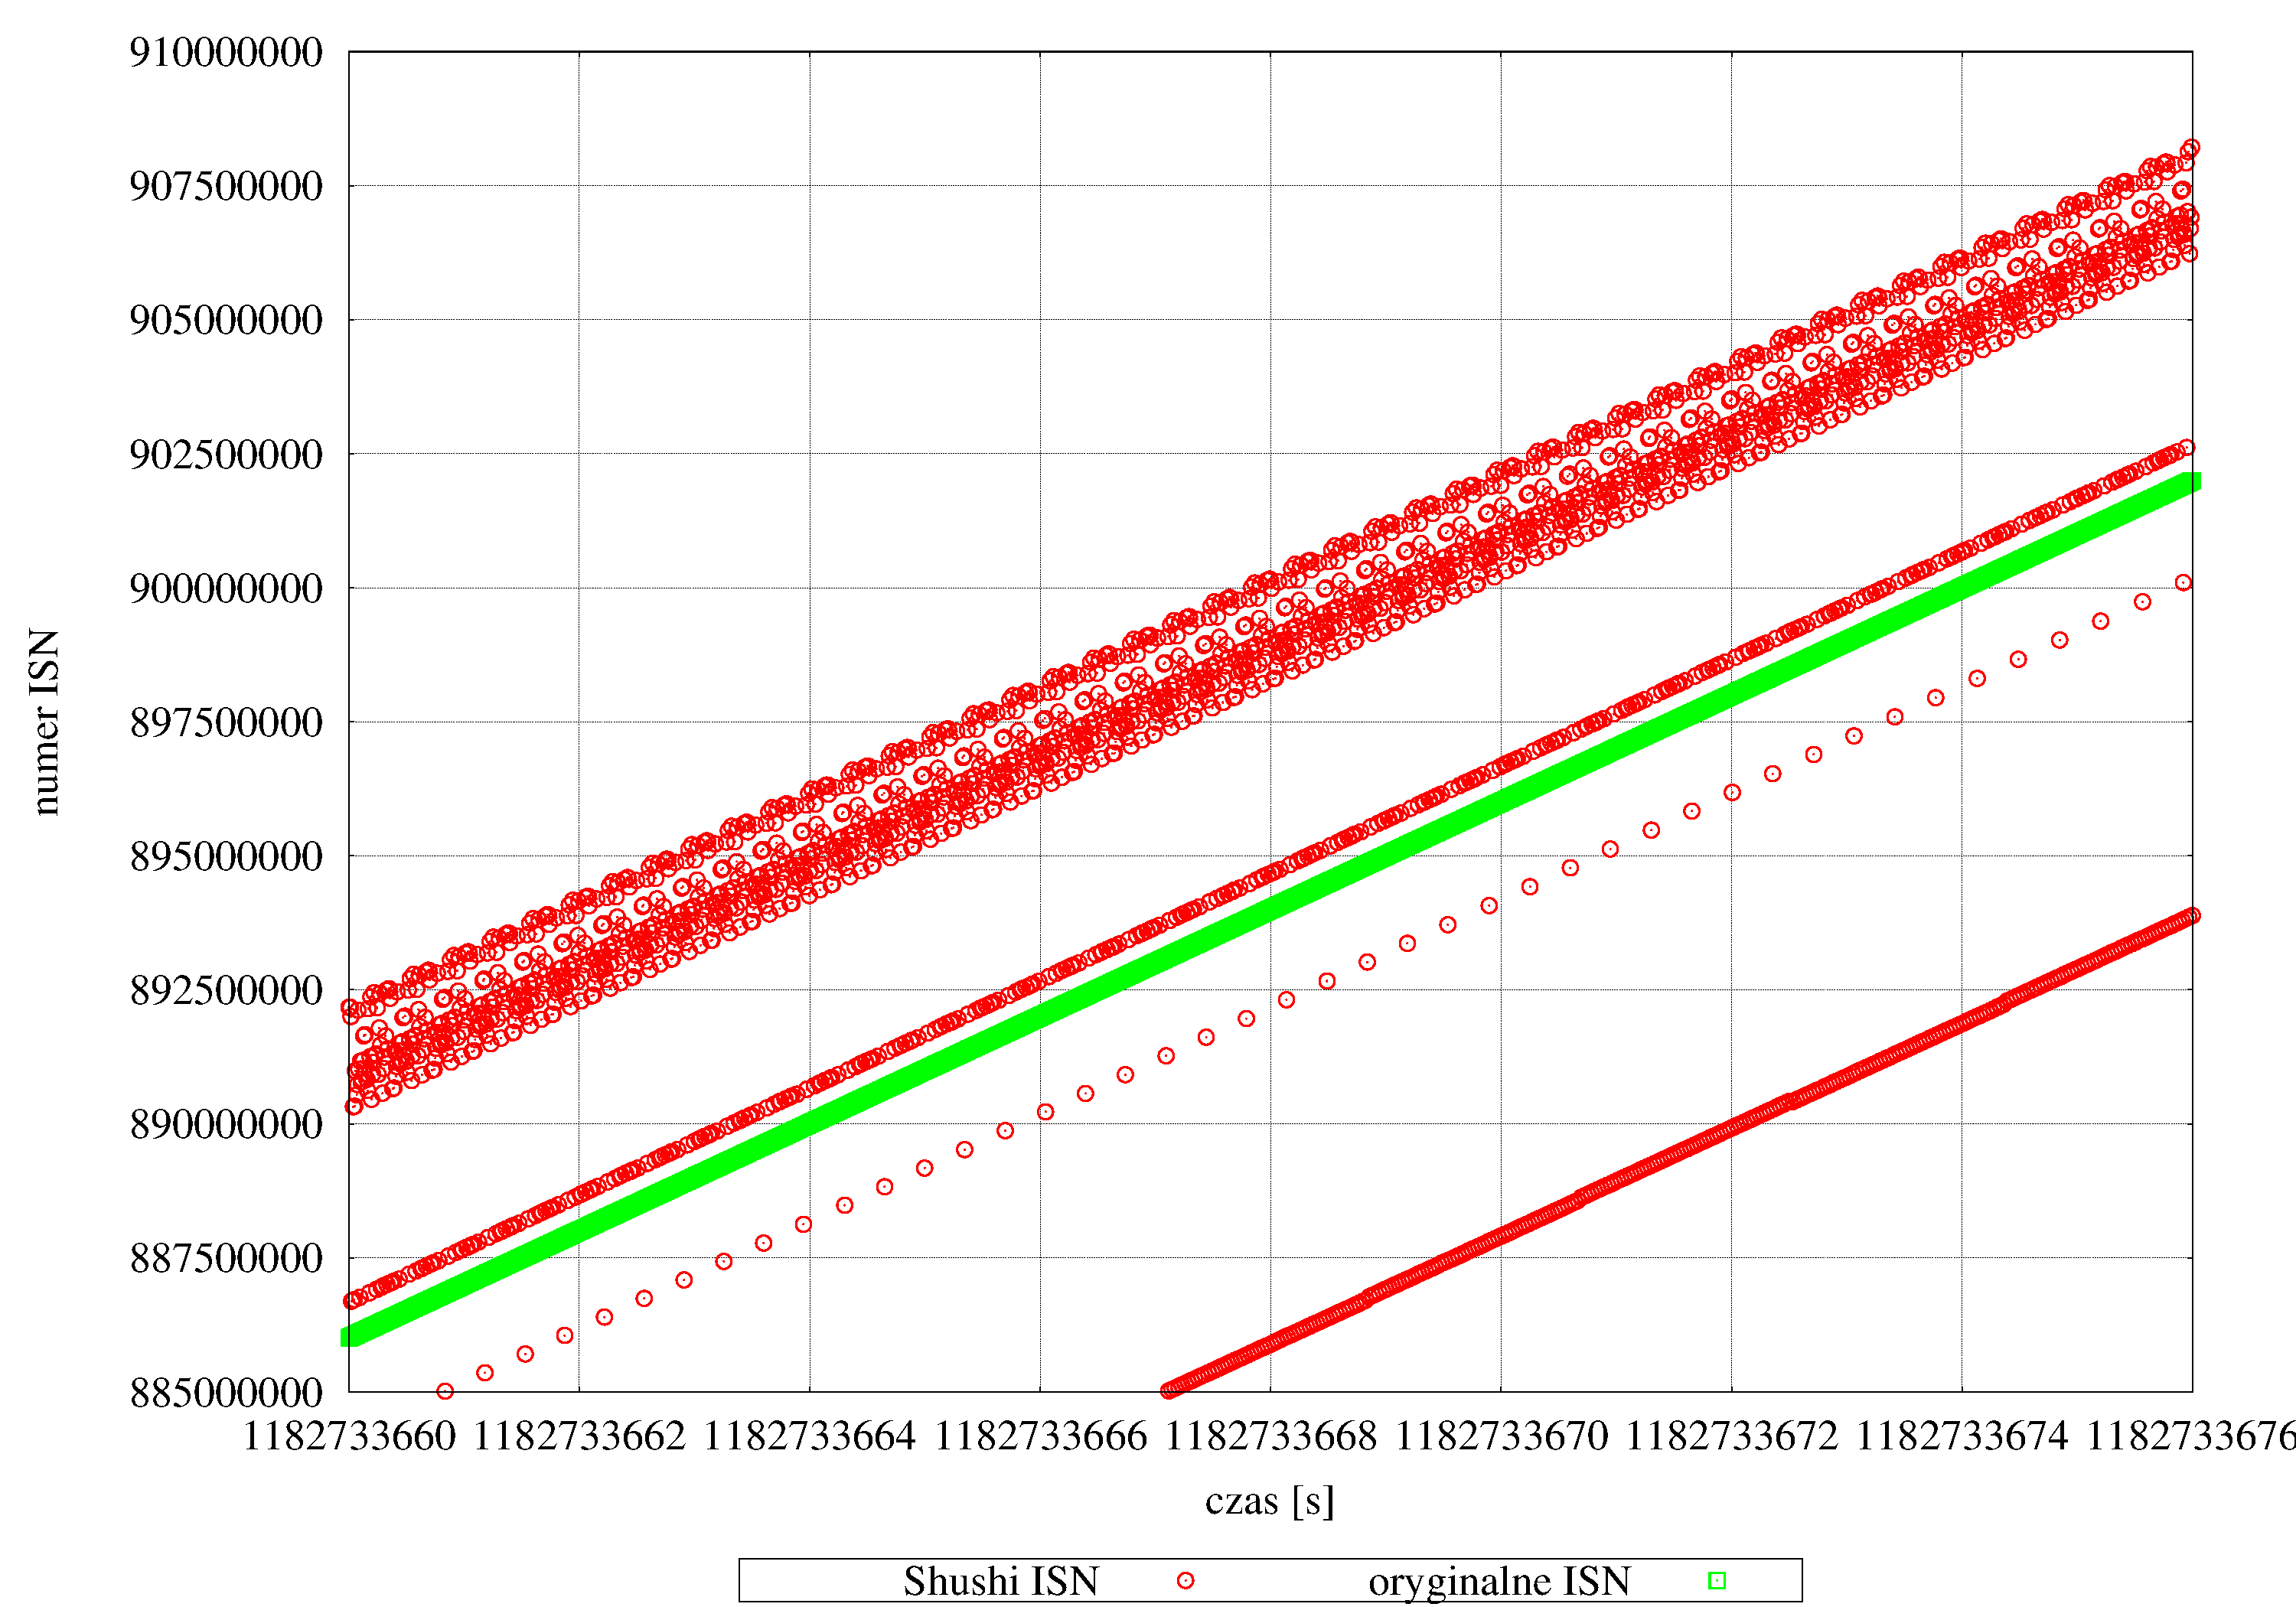
\includegraphics[scale=0.21]{\ImgPath/rys/IPPortConstData.pdf}
    \end{center}
    \caption{Numery ISN wygenerowane przez jądro oraz \tech{Shushi}, stałe
    numery IP oraz porty TCP, stałe dane dla \tech{Shushi}, serie po około 2800
    próbek.}
    \label{IPPortConstData}
\end{figure}

\begin{figure}[!htbp]
    \begin{center}
        \centering
        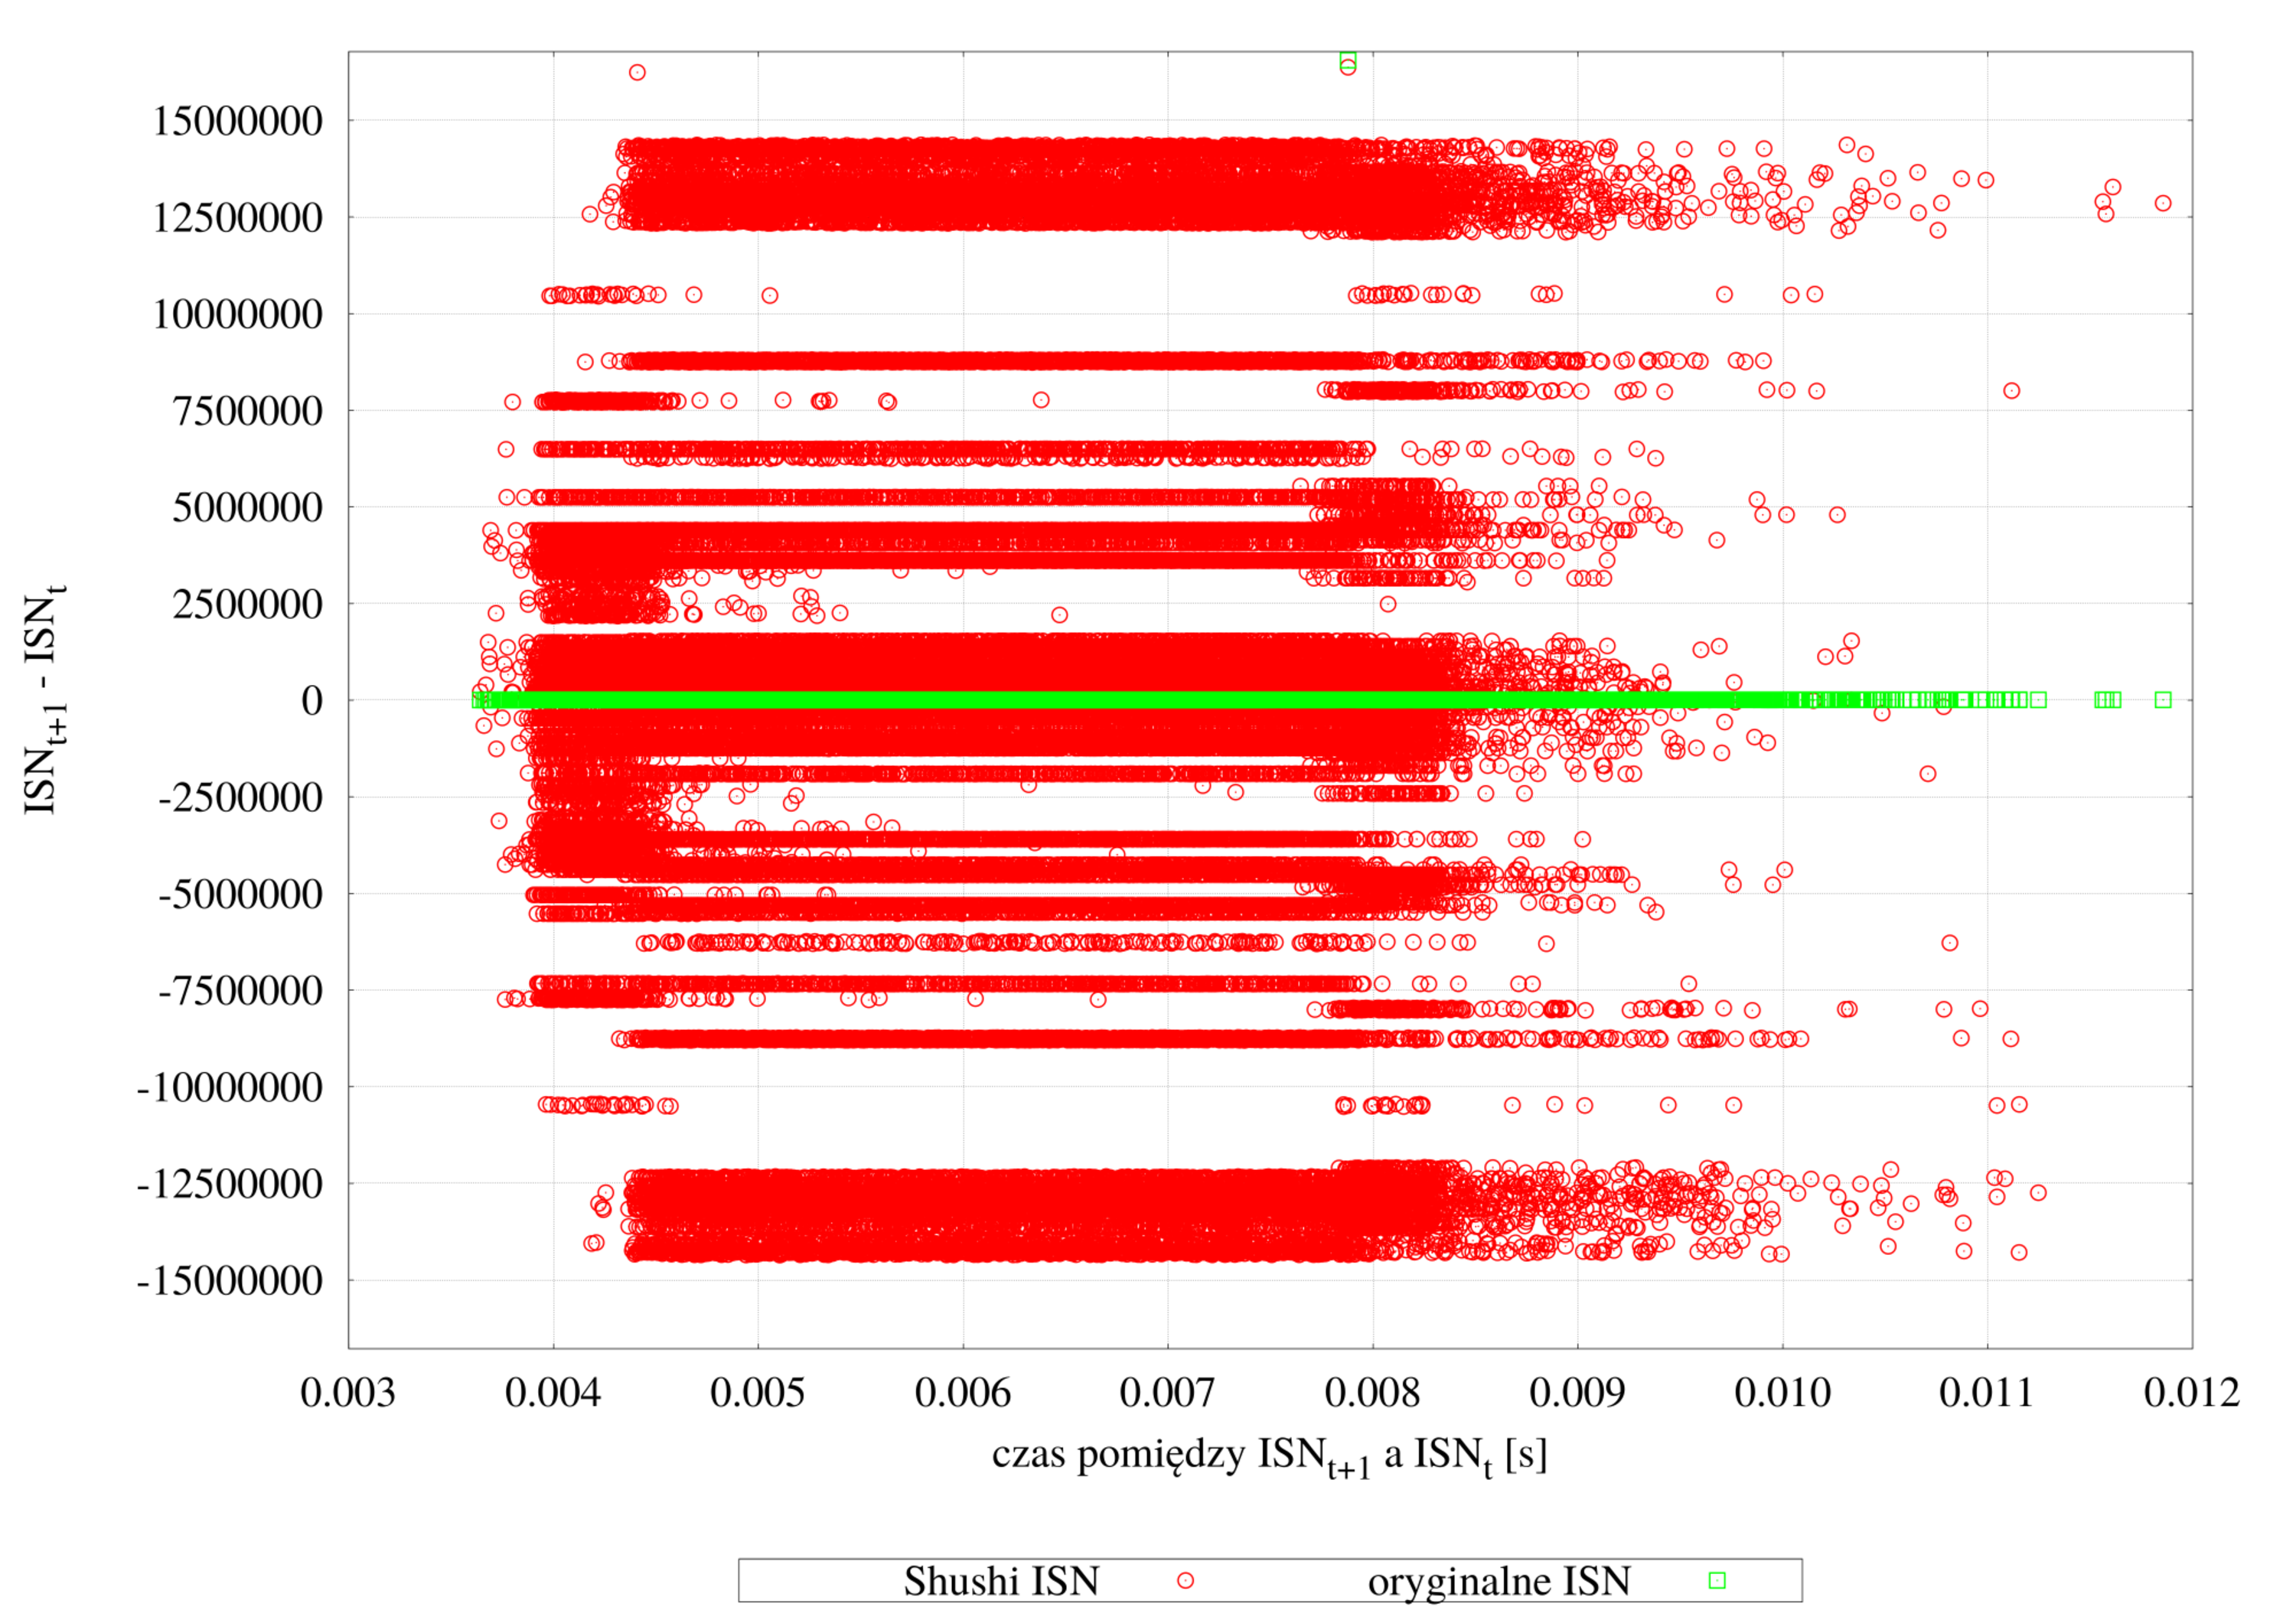
\includegraphics[scale=0.21]{\ImgPath/rys/IPPortConstDataDiff.pdf}
    \end{center}
    \caption{Różnice pomiędzy kolejnymi numerami ISN wygenerowanymi przez
    jądro oraz \tech{Shushi}, stałe numery IP oraz porty TCP, stałe dane dla
    \tech{Shushi}, serie po około 60000 próbek.}
    \label{IPPortConstDataDiff}
\end{figure}

\begin{figure}[!htbp]
    \begin{center}
        \centering
        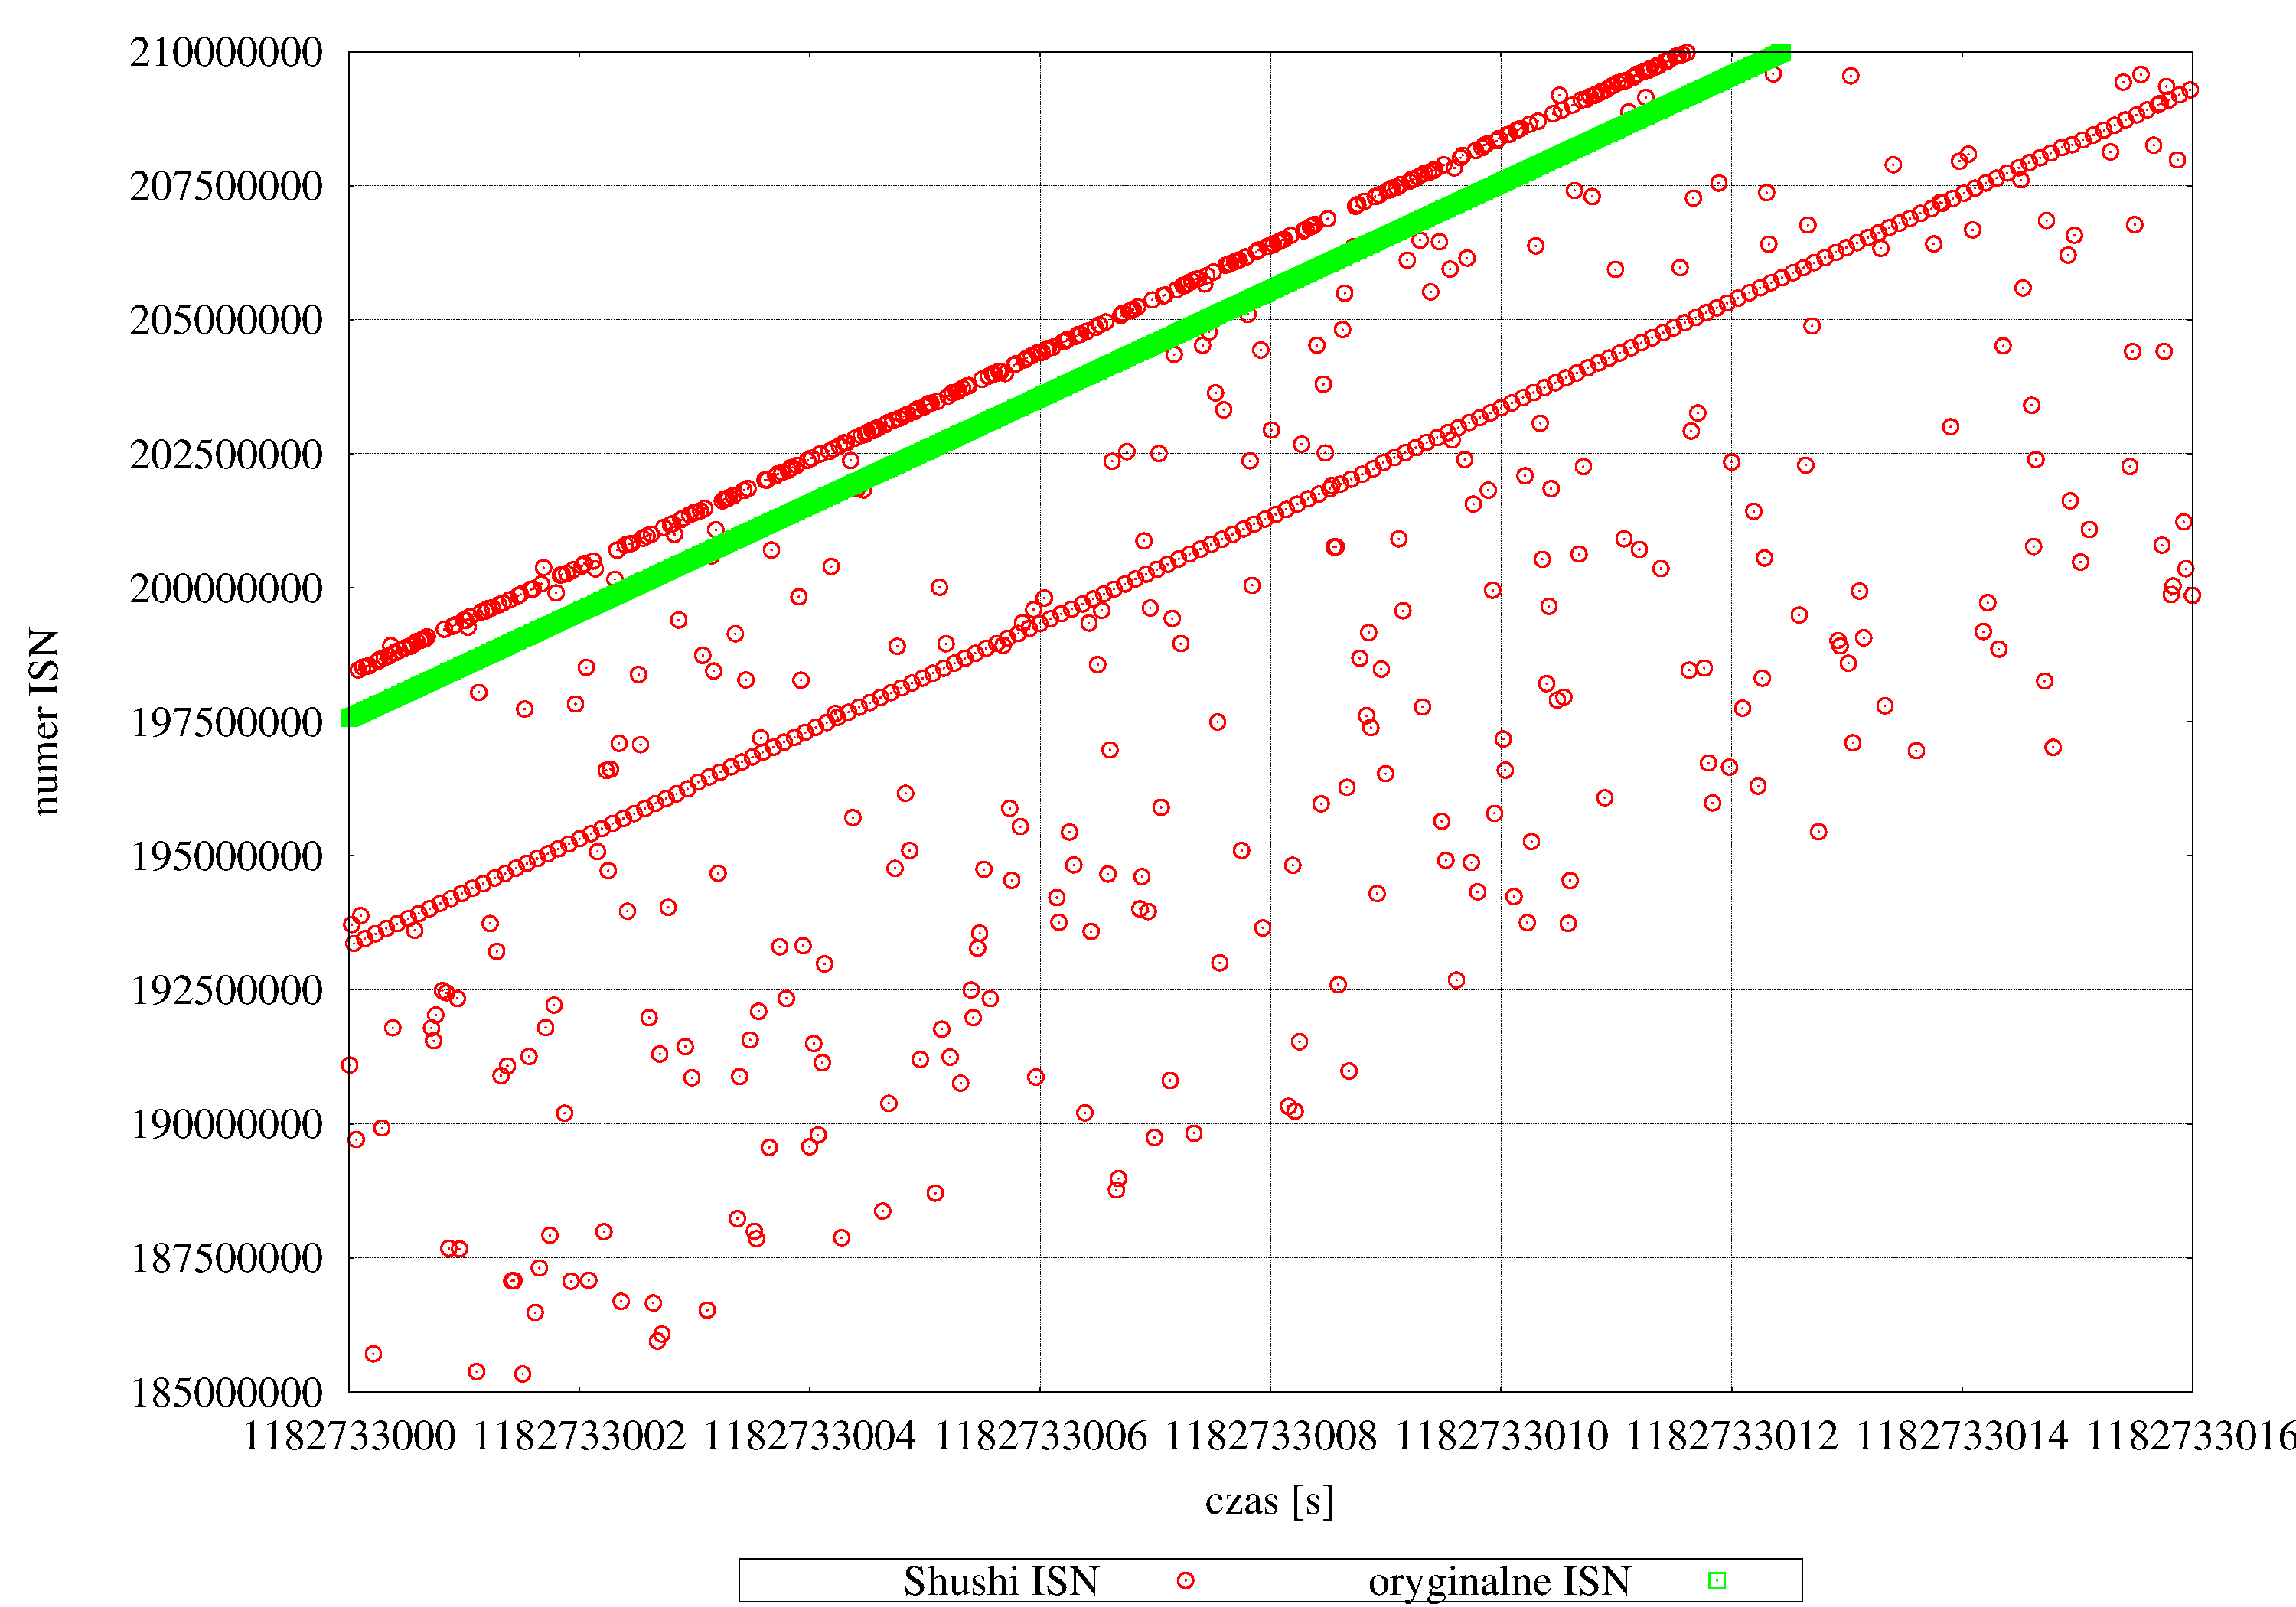
\includegraphics[scale=0.21]{\ImgPath/rys/IPPortRandData.pdf}
    \end{center}
    \caption{Numery ISN wygenerowane przez jądro oraz \tech{Shushi}, stałe
    numery IP oraz porty TCP, losowe dane dla \tech{Shushi}, serie po około 860
    próbek.}
    \label{IPPortRandData}
\end{figure}

\begin{figure}[!htbp]
    \begin{center}
        \centering
        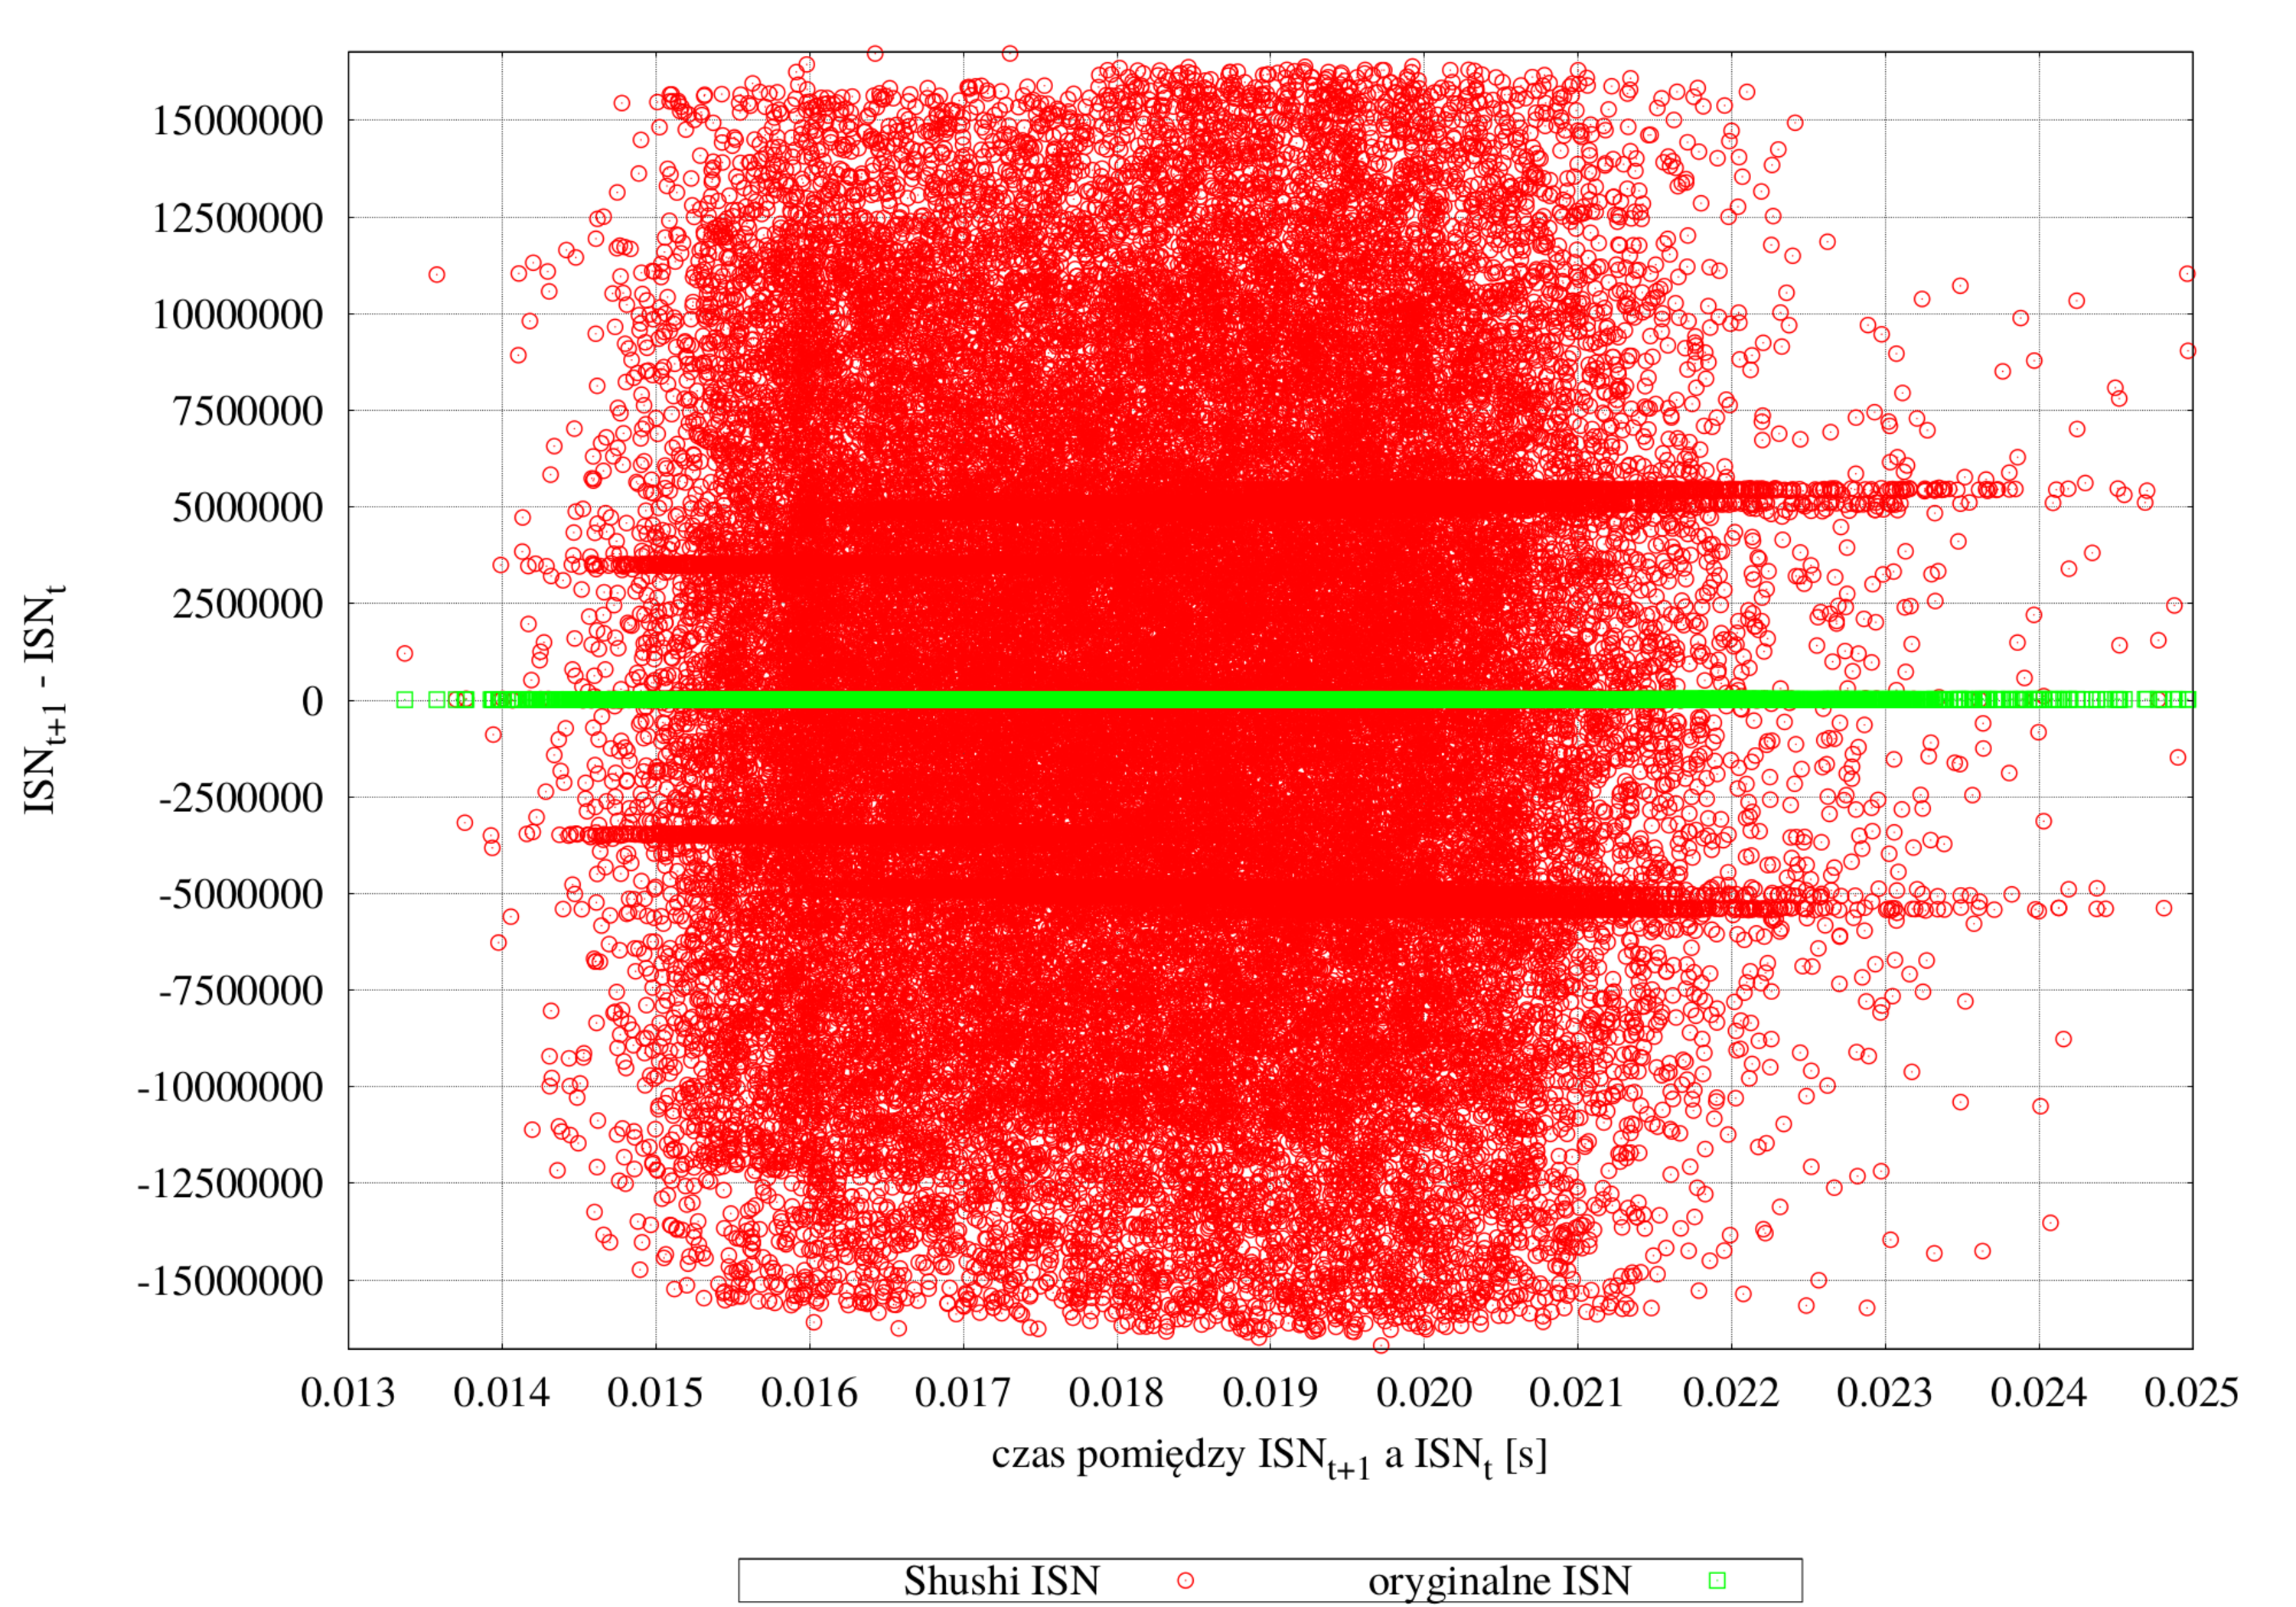
\includegraphics[scale=0.21]{\ImgPath/rys/IPPortRandDataDiff.pdf}
    \end{center}
    \caption{Różnice pomiędzy kolejnymi numerami ISN wygenerowanymi przez
    jądro oraz \tech{Shushi}, stałe numery IP oraz porty TCP, losowe dane dla
    \tech{Shushi}, serie po około 60000 próbek.}
    \label{IPPortRandDataDiff}
\end{figure}

\begin{thebibliography}{99}
    \addcontentsline{toc}{chapter}{Bibliografia}
    \bibitem{Stevens}{W. R. Stevens, G. R. Wright, ,,Biblia TCP/IP tom 1'', RM,
    1998.}
    \bibitem{USDoD}{U. S. Department Of Defense, ,,Trusted Computer System
    Evaluation Criteria'', 1985.}
    \bibitem{FirstCC}{B. W. Lampson, ,,A note on the confinment problem'', w ,,Proc.
    of the Communications of the ACM'', październik 1973, numer 16:10,\newline
    strony 613-615.}
    \bibitem{PrisonersProblem}{G. J. Simmons, ,,The prisoners' problem and the
    subliminal channel'', w ,,Advances in Cryptology: Proceedings of Crypto 83 (D.
    Chaum, ed.)'', strony 51-67, Plenum Press, 1984.}
    \bibitem{Kerckhoff}{ A. Kerckhoffs, ,,La Cryptographie Militaire (Military
    Cryptography)'', J. Sciences Militaires, luty 1883.}
    \bibitem{Hanssen}{A. Havill, ,,The Spy Who Stayed Out In The Cold: The Secret
    Life of Double Agent Robert Hanssen'', St. Martin's Press, 2001.}
    \bibitem{schematKomunikacjiPrzypis}{C.Cachin, ,,An Information-Theoretic Model
    for Steganography'', w ,,Information and Computation'', 4 marzec 2004.}
    \bibitem{SweetyPresentation}{S.Chauhan, ,,Embedding Covert Channels into
    TCP/IP'', 7th Information Hiding Workshop, czerwiec 2005.}
    \bibitem{RFC793}{Information Sciences Institute, University of Southern
    California, ,,Transmission Control Protocol'', RFC793, wrzesień 1981.}
    \bibitem{RFC1323}{V. Jacobson, R. Braden, D. Borman, ,,TCP extensions for high
    performance'', RFC1323, maj 1992.}
    \bibitem{RFC1948}{S. Bellovin, ,,Defending against sequence number attacks.'',
    RFC1948, IETF, 1996.}
    \bibitem{RFC2960}{R. Stewart, Q. Xie, K. Morneault, C. Sharp, H. Schwarzbauer,
    T. Taylor, I. Rytina, M. Kalla, L. Zhang, V. Paxson, „Stream Control
    Transmission Protocol”, RFC2960, Network Working Group, październik 2000.}
    \bibitem{Rowland}{C. H. Rowland, ,,Covert Channels in the TCP/IP Protocol
    Suite'', First Monday, 1997. \newline
    \url{http://www.firstmonday.dk/issues/issue2\_5/rowland/}}
    \bibitem{LOKI}{Alhambra, daemon9, ,,Project Loki: ICMP Tunneling'', Phrack
    Magazine, Issue 49. \url{http://phrack.org}}
    \bibitem{LOKI2}{daemon9, ,,LOKI2'', Phrack Magazine, Issue 51.
    \url{http://phrack.org}}
    \bibitem{RWWWS}{van Hauser, Reverse WWW Shell, THC, The Hacker's
    Choice.\newline \url{www.thc.org}}
    \bibitem{CCdetectionSVM}{T. Sohn, J. Seo, J. Moon, ,,A Study on the Covert
    Channel Detection of TCP/IP Header Using Support Vector Machine'', Volume 2836
    of Lecture Notes in Computer Science., Springer-Verlag (2003) 313-324.}
    \bibitem{LOKIdetectionSVM}{T. Sohn, T. Noh, J. Moon, ,,Support Vector Machine
    Based ICMP Covert Channel Attack Detection'', Volume 2836 of Lecture Notes in
    Computer Science., Springer-Verlag, 2003, strony 461-464.}
    \bibitem{devcc}{J. Giffin, R. Greenstadt, P. Litwack, R. Tibbetts, ,,Covert
    messaging in TCP'', w Dingledine, Privacy Enhancing Technologies. Volume 2482 of
    Lecture Notes in Computer Science., Springer-Verlag (2002) 194-208.
    \url{http://www.mit.edu/\textasciitilde gif/covert-channel/}}
    \bibitem{ActiveWardens}{G. Fisk, M. Fisk, Ch. Papadopoulos, J. Neil,
    ,,Eliminating Steganography in Internet Traffic with Active Wardens'', 5th
    International Workshop on Information Hiding, październik 2002.}
    \bibitem{JR}{J. Rutkowska, ,,The Implementation of Passive Covert Channels in
    Linux Kernel'', Chaos Communication Congress, grudzień 2004.}
    \bibitem{LinuxNetwork}{Ch. Benvenuti, ,,Understanding Linux Network Internals'',
    O'Reilly,\newline grudzień 2005.}
    \bibitem{p55}{kossak, ,,Building Into The Linux Network Layer'', Phrack
    Magazine, Issue 55. \url{http://phrack.org}}
    \bibitem{ML}{Steven J.Murdoch and Stephen Lewis, ,,Embedding Covert Channels
    into TCP/IP'', University of Cambridge, Computer Laboratory,\newline 29 lipec
    2005.}
    \bibitem{NvsNN}{Eugene Tumoian, Maxim Anikeev, ,,Detecting NUSHU Covert Channels
    Using Neural Networks'', Taganrog State University of Radio Engineering,
    Department of Information Security.}
    \bibitem{p58}{mayhem, ,,IA32 Advanced Function Hooking'', Phrack
    Magazine,\newline Issue 58. \url{http://phrack.org}}
    \bibitem{p61}{bioforge, ,,Hacking the Linux Kernel Network Stack'', Phrack
    Magazine, Issue 61. \url{http://phrack.org}}
    \bibitem{kernelMEM}{Robert Love, ,,Kernel Korner - Allocating Memory in the
    Kernel'',\newline 1 grudzień 2003.}

\end{thebibliography}

\zakonczenie  % wklejenie recenzji i opinii

\end{document}
%+++ END +++
